\pagenumbering{arabic}
%\setcounter{page}{1}
\setcounter{chapter}{7}
\chapter{One Sample Confidence Intervals On a Proportion}
\index{Introduction}
\label{sec.matrix}
%start relabeling as 2.1 etc
\pagestyle{myheadings}  \markboth{\ref{sec.matrix}.
\titleref{sec.matrix}}{}
%\setcounter{equation}{0}

Perviously, we have introduced confidence interval based on known and unknown variance. Moreover, confidence intervals are also applied to an unknown population parameter. For example, suppose we are interested the proportion of total number of left-handed students among all students who are currently studying at University of Toronto Mississauga. The question is: how do we know such the parameter which estimates the proportion of left-handed students at UTM? While, it is impossible to proceed it directly by counting both the total number of students and all left-handed students at UTM. Then, we have to work with confidence intervals.\\

\noindent
Firstly, we take a random sample of students at UTM, then we calculate how many students are left-handed by dividing total number of left-handed students in that sample with total number of students in it, and denote the proportion as $\hat{p}$. Next we begin our confidence interval calculation to get a range of number with a certain level of confidence.\\

\noindent
Now let's begin with the proper definition of confidence interval on proportion.

\begin{definition}[One Sample Confidence Intervals On a Proportion]
We select a random sample of size $n$ from a population with \textbf{unknown} proportion $p$ of success. An approximate confidence interval for \textbf{p} is: \[ p = \hat{p}  \pm z_{\frac{\alpha}{2}} \cdot \sqrt{\frac{\hat{p}(1 - \hat{p})}{n}}, \text{ where $\hat{p} = \frac{\text{number of observations satisfying the criteria}}{n}$.}\]
To apply this confidence interval, there are $3$ conditions that we need to guarantee:
\begin{itemize}
	\item $1$. Random sample;
	\item $2$. Independent and identically distributed Bernoulli trails;
	\item $3$. We have a large chosen sample size ($n\hat{p} \ge 10$ and $n(1-\hat{p}) \ge 10$).
\end{itemize}
\end{definition}

\noindent
A good way to understand confidence interval is visualization. Now, suppose we have a valid estimation $\hat{p}$. After the entire procedure of confidence interval, our population proportion ($p$) should be as the following number line shows:\\

\begin{center}
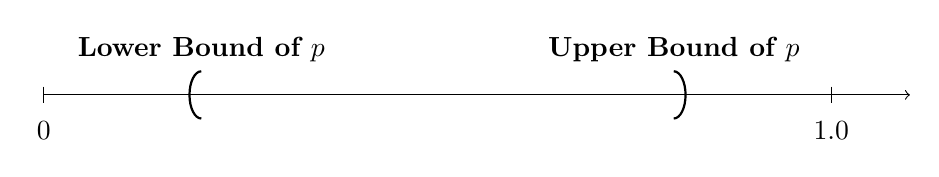
\begin{tikzpicture}
  \draw[->] (0,0) -- (11,0);
  \foreach \x in {0, 1.0} {
    \draw[shift={(\x*10,0)},color=black] (0pt,3pt) -- (0pt,-3pt);
    \draw[shift={(\x*10,0)},color=black] (0pt,-6pt) node[below] {\x};}
  \draw[thick] (2.0,-0.3) arc (270:90:0.15cm and 0.3cm);
  \node[above] at (2.0,0.3) {\textbf{Lower Bound of $p$}};
  \draw[thick] (8.0,-0.3) arc (-90:90:0.15cm and 0.3cm);
  \node[above] at (8.0,0.3) {\textbf{Upper Bound of $p$}};
\end{tikzpicture}
\end{center}

\noindent
Remember that your final answer of the range of $p$ must between $0$ and $1$, since we are working with proportion.


